% !TeX root = ../sustechthesis-example.tex

\chapter{引\quad 言}
\section{研究背景与意义}
细长杆、薄板薄壳等结构在外载荷作用下会发生结构失稳屈曲\cite{BAZANT200055,bazant2010stability}。在传统意义上,结构失稳被视为一种需要避免的现象,因为失稳通常意味着结构的失效、功能丧失甚至灾难性后果。例如,在建筑工程中,梁杆的屈曲失稳可能导致建筑物,桥梁的坍塌;在航空航天领域,机翼或壳体的失稳可能引发飞行事故。

对于细长结构和薄壁结构,在载荷作用下往往可以发生很大的位移以及旋转,同时其应变仍保持小应变状态,即结构在展现出明显的几何非线性的同时材料保持在线性范围且不发生失效。当此类柔性结构处于后屈曲阶段时,往往展示出了丰富的非线性行为,如多稳态行为及不同稳态构形之间的突跳行为。基于此,近年来研究者开始将这类柔性结构的失稳行为视为设计具有新型功能结构的机会,而非结构发生失效破坏的源头\cite{10.1115/1.4031456}。通过对结构精确设计和控制失稳行为,从而赋予结构全新的力学特性,如利用柔性结构的后屈曲行为来设计展开结构,自适应结构,超材料,柔性机器人以及将其应用于柔性电子设备中。

近年来,研究者们在利用结构失稳实现新特性方面取得了一系列重要进展,如图~\ref{fig:1}所示。在结构设计领域,研究者利用结构的后屈曲特性来设计展开结构,发展自适应结构。展开结构的初始构形通常为高度紧致的折叠状态。在外部激励(如机械力、热激励或电激励)的作用下,这些结构能够通过特定的变形机制从二维平面状态或紧凑的三维状态转变为大尺度的空间三维构形。其中一种展开方式为处于平面二维状态的结构在受到特定的外力时会产生面外屈曲,从而展开为三维构形\cite{panetta2019x,chen2021bistable,liu2023deployable,10.1145/3386569.3392490,yu2023continuous}。
自适应结构能够根据载荷条件的变化,自动调整形态与行为,来优化其性能或维持功能。例如,在航空领域一些研究者利用复合材料来制造多稳态翼型,这些翼型可以自主切换构形来适应不同的气动载荷\cite{arrieta2013modelling,DIACONU2008689}。由于这些结构具有轻量化,智能化(可自适应外界条件)等特点,因此被广泛应用于各种工程领域,如航空航天\cite{zhang2021deployable},土木建筑\cite{GEIGER20208363}。
在超材料(metamaterials)领域,通过设计周期性微结构并利用其失稳行为,可以实现负泊松比、负刚度和可编程力学性能等奇异特性\cite{cui2014coding}。这些超材料在冲击防护、振动隔离和能量吸收等方面展现出巨大的应用潜力。
在机器人设计领域,一些微小型机器人利用柔性结构的突跳行为来为机器人提供驱动力,例如双稳态结构在两个稳态之间的突跳可以为游泳机器人提供动力\cite{chen2018harnessing,chi2022snapping}。
\begin{figure}
	\centering
	\subcaptionbox{展开结构\cite{10.1145/3386569.3392490}\label{fig:1_1}}
	{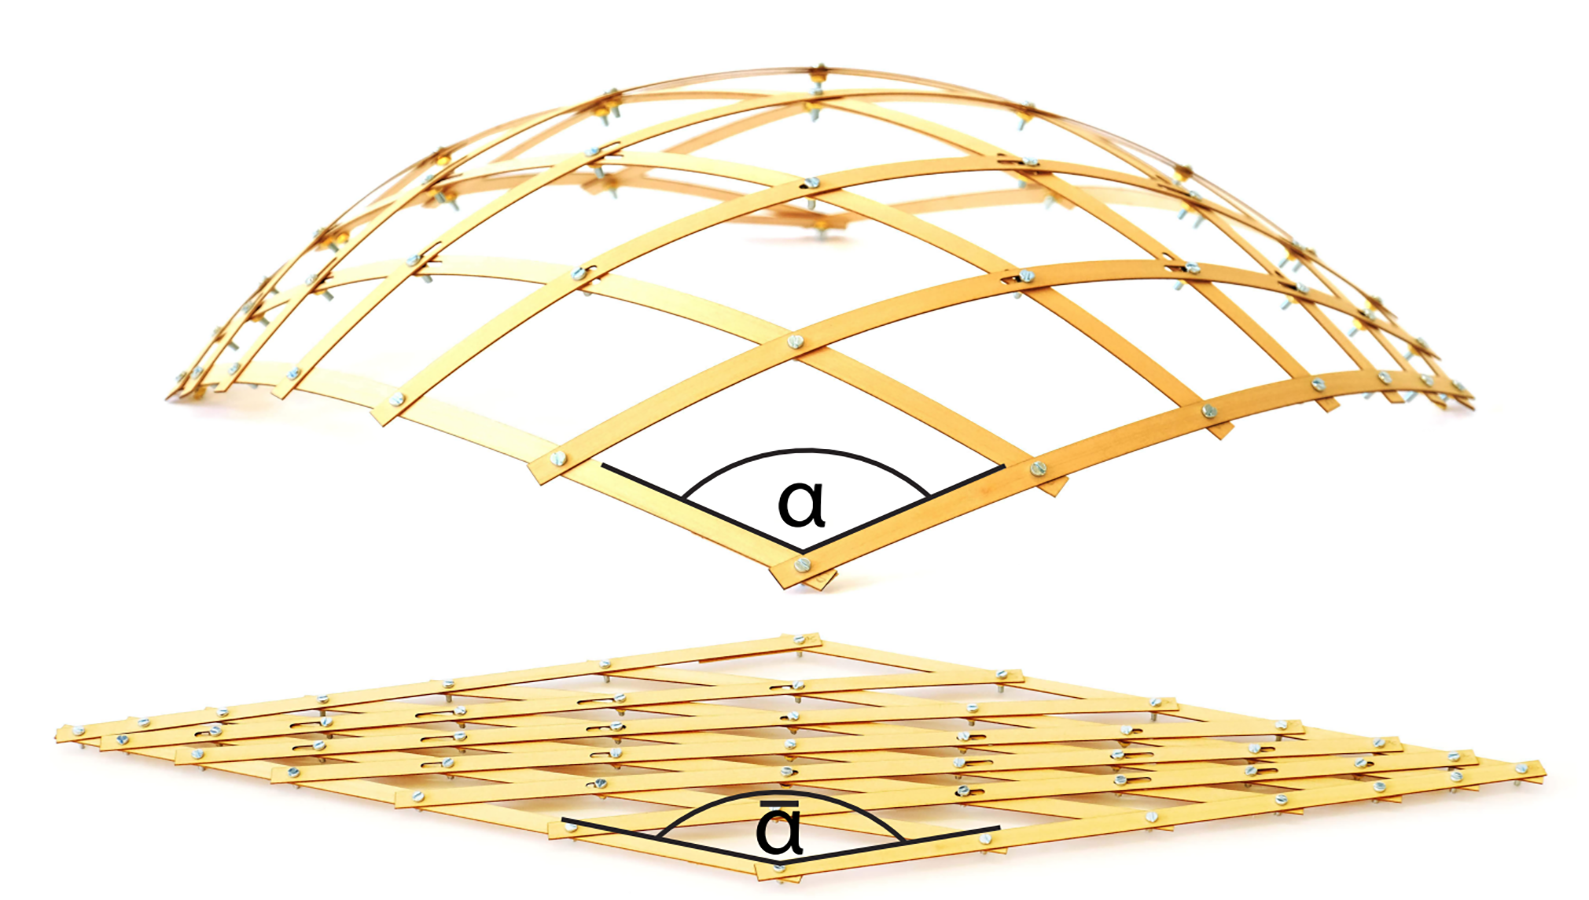
\includegraphics[width=0.49\linewidth]{1_1(1).png}}
	\subcaptionbox{不同载荷下的二维格状蜂窝超材料\cite{PhysRevLett.99.084301}\label{fig:1_2}}
	{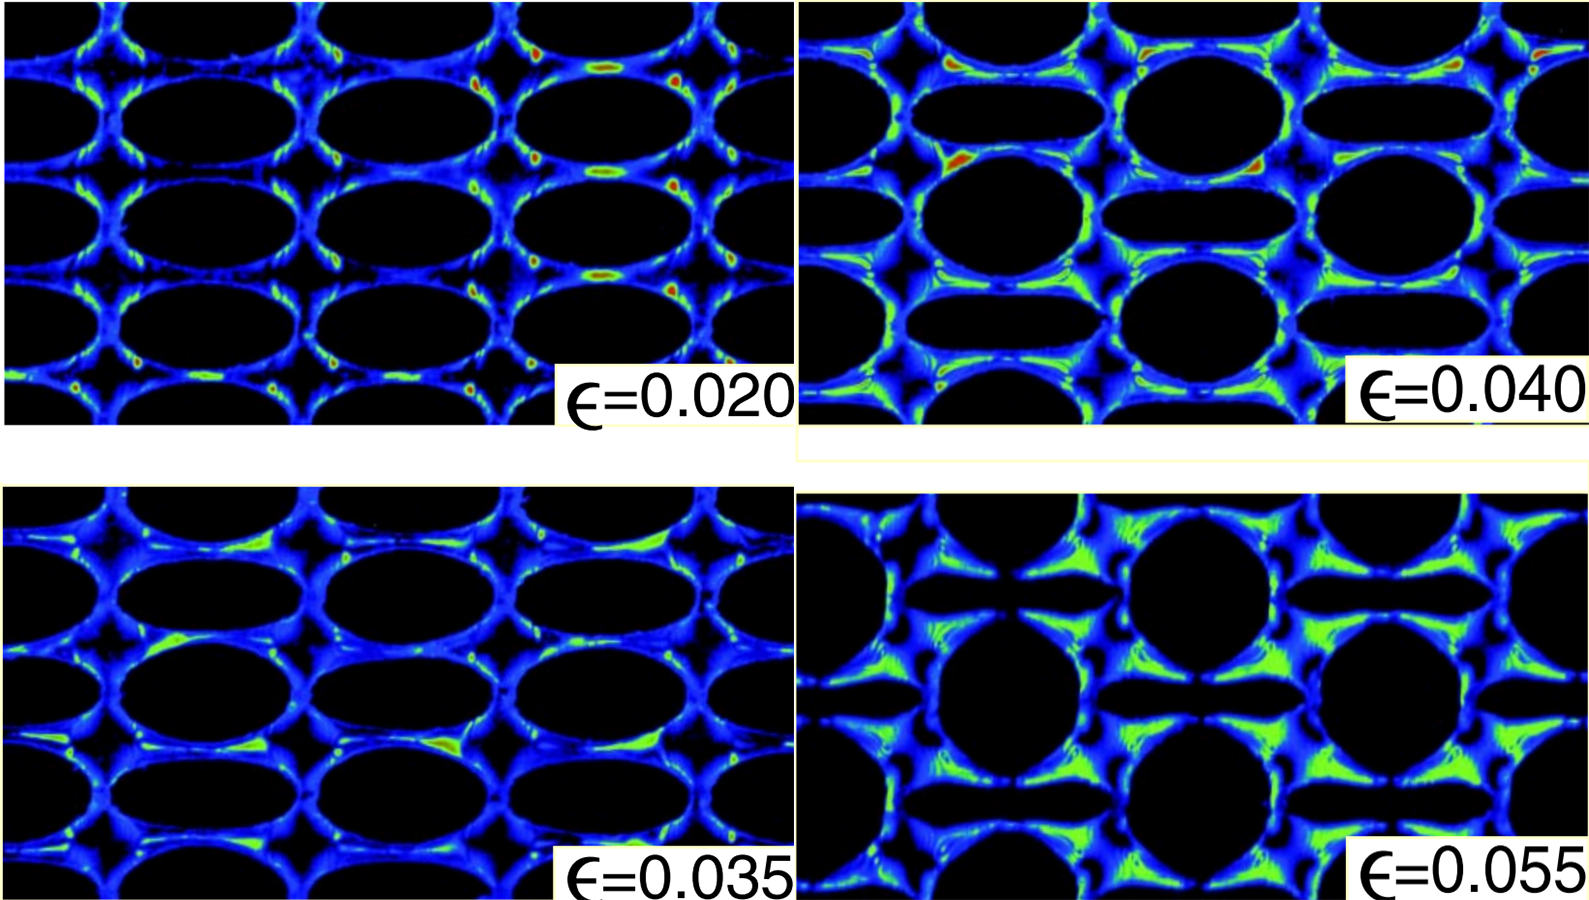
\includegraphics[width=0.49\linewidth]{1_1(2).png}}\\
	\subcaptionbox{双稳态负泊松比结构\cite{chen2021bistable}\label{fig:1_3}}
	{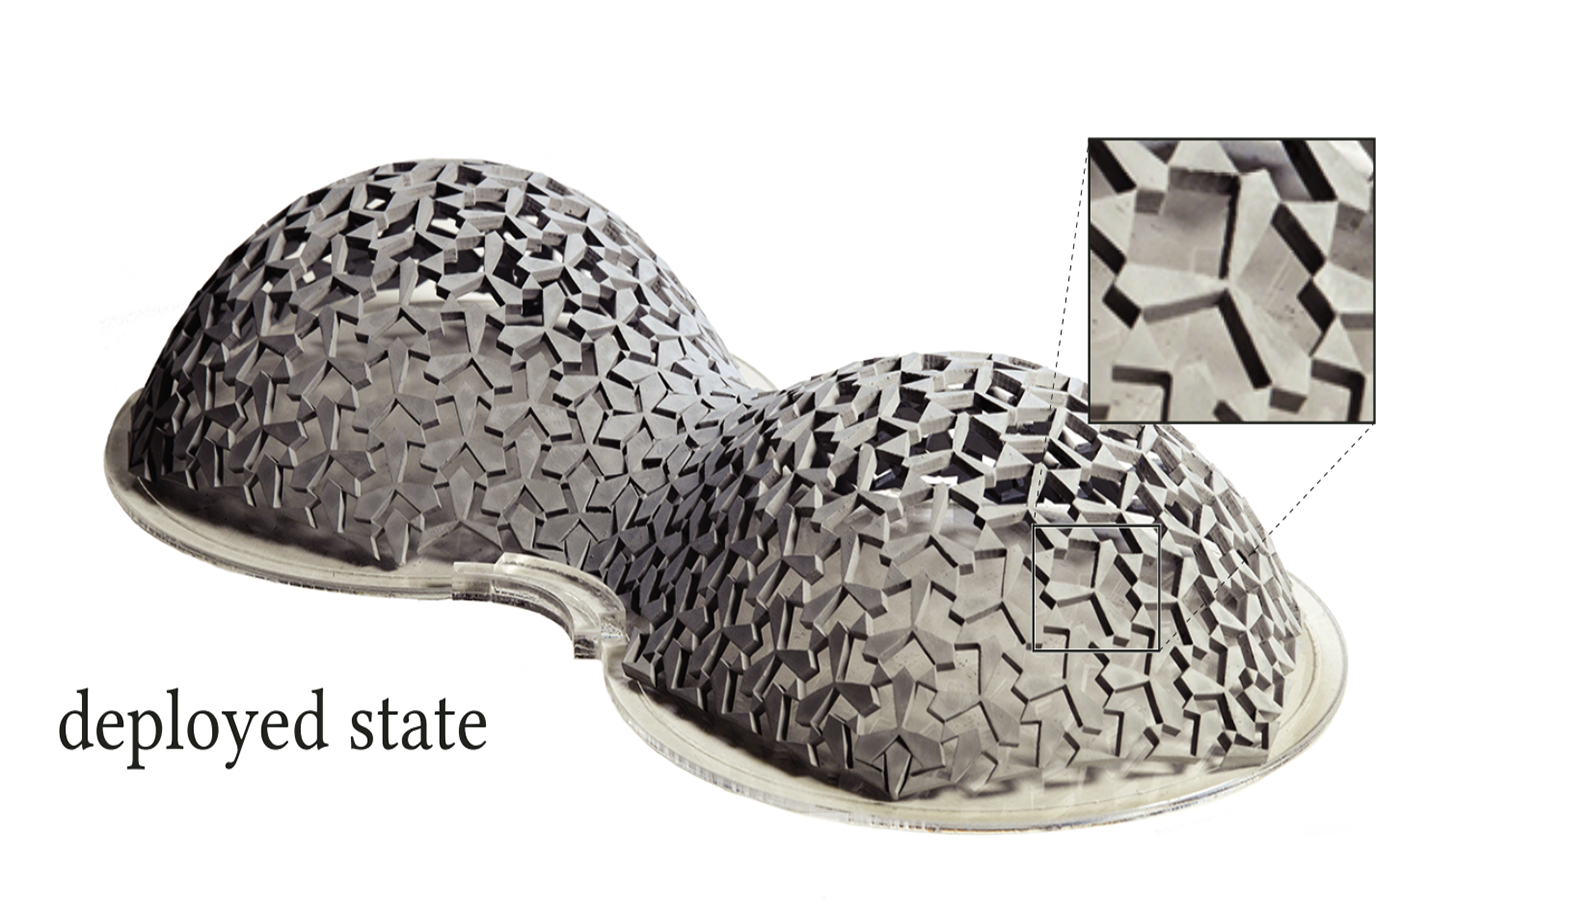
\includegraphics[width=0.49\linewidth]{1_1(3).png}}
	\subcaptionbox{无系链游泳机器人\cite{chen2018harnessing}\label{fig:1_4}}
	{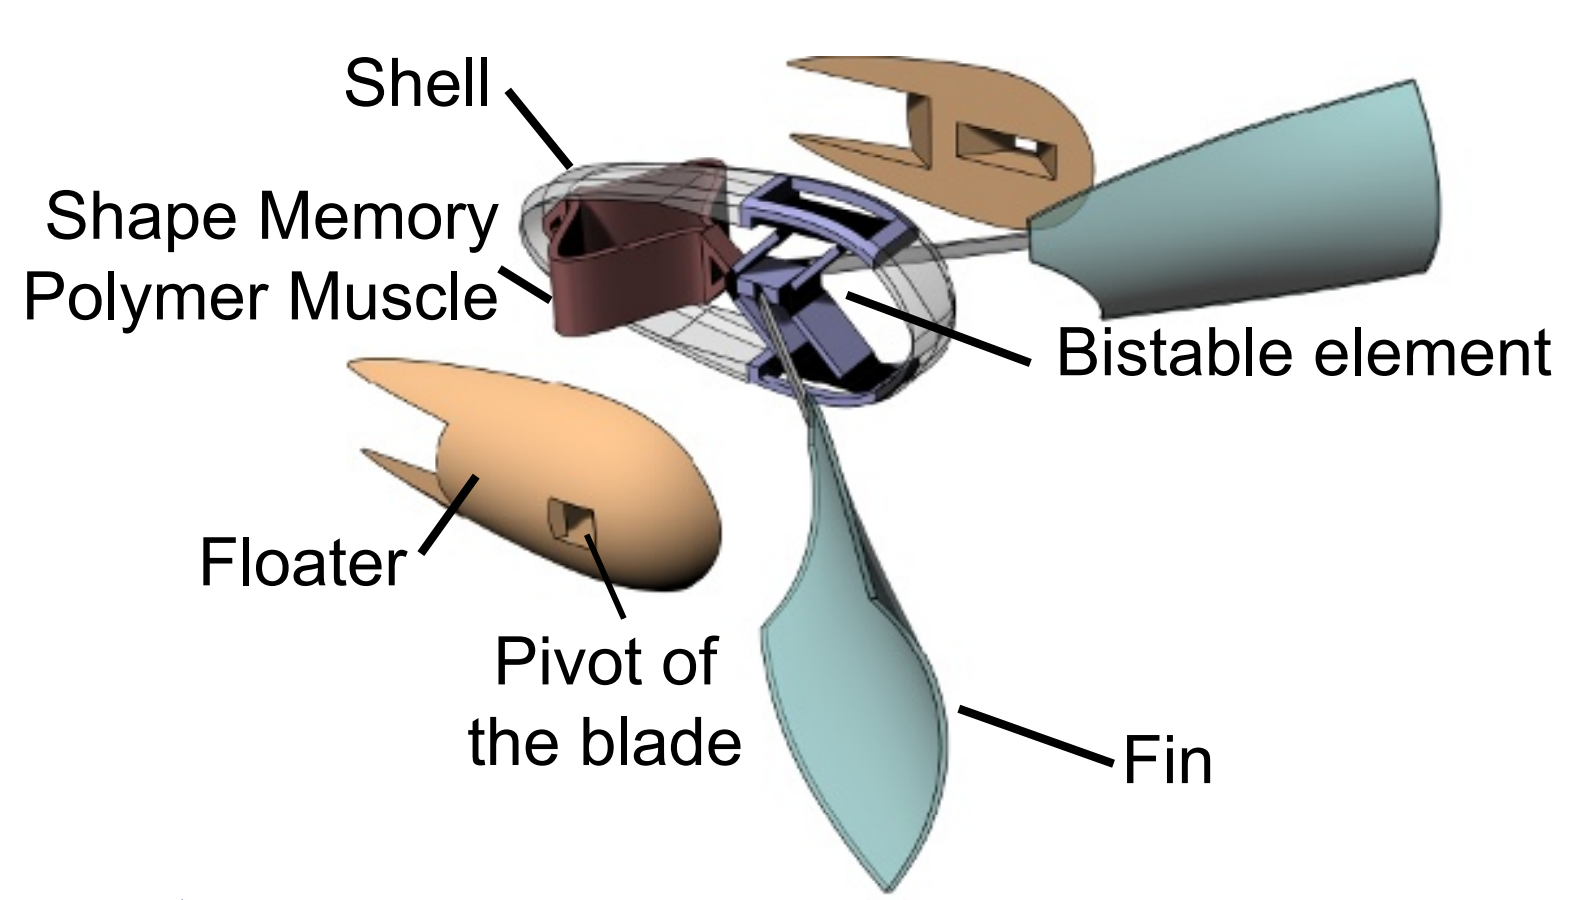
\includegraphics[width=0.49\linewidth]{1_1(4).png}}
	\caption{结构失稳在展开结构,超材料以及机器人领域的应用}
	\label{fig:1}
\end{figure}

另一方面,对柔性结构的屈曲失稳研究为柔性电子设备的设计与制造提供了力学基础。相比于传统的电子设备,柔性电子设备可以更好的贴合复杂曲面以及进行动态变形来适应不同的应用场景,此外柔性电子设备往往使用超薄材料来设计,因此具有轻质化和薄型化的特点。基于上述特点与优势,柔性电子设备展现出了越来越重要的应用前景,包括可穿戴的通讯系统,佩戴式健康监测设备,可嵌入人体的治疗疾病设备,机器人柔性皮肤\cite{rogers2010materials}等。为了制造这些柔性电子设备,近年来发展了许多重要技术,其中平面印刷技术\cite{yin2020structural}(planar printing techniques)通过利用结构的屈曲失稳行为来制备柔性电子设备,该技术由于其相对于其他技术的简单性而被广泛应用。平面印刷技术大致可以分为三类:基底设计技术,三维组装技术,蛇形设计与岛桥结构。

在基底设计技术\cite{bowden1998spontaneous}中,首先对柔软基底进行预处理(如拉伸或加热处理)以在基底中引入预应力。随后,将电子器件安置在预处理后的柔性基底上。当基底释放预应力时,基底自身的变形会对电子器件施加压力,导致电子器件发生面外屈曲,形成稳定的褶皱形貌。这种褶皱结构为结构提供了更多可拉伸空间,从而显著增强了电子设备的可拉伸性和机械耐久性。相比之下,三维组装技术则更为复杂,需要对基底进行精确加工以实现特定的预应力分布,并通过精确设计电子器件的二维初始构形及其与基底的粘接区域,将二维电子器件转换为目标三维构形\cite{cheng2023programming}。这种技术不仅依赖于基底的力学特性,还需要对器件的几何形状和材料性能进行精细调控,以实现复杂的三维结构。“岛—桥”结构\cite{zhang2013buckling},如图~\ref{fig:1_2v}所示,为柔性电子设备制造的另外一类方法。该方法中,整个电子设备被安置到可变形的基底上,在基底上排布一系列小的刚性底片(island)用以布置设备的主要部件,并将每个小的刚性底片利用可承受较大变形的连接部件(bridge)进行连接,实现不同基底之间的通信和电传导。对于这一类布局,其用以安装电子功能元器件的小刚片单元往往为刚性结构,整个设备的可拉伸性取决于连接部件的可拉伸性,其中一种被广泛应用于柔性电子的连接部件为蛇形结构\cite{li2005compliant},如图~\ref{fig:1_2v}中下方黑色曲线所示。
\begin{figure}
	\centering
	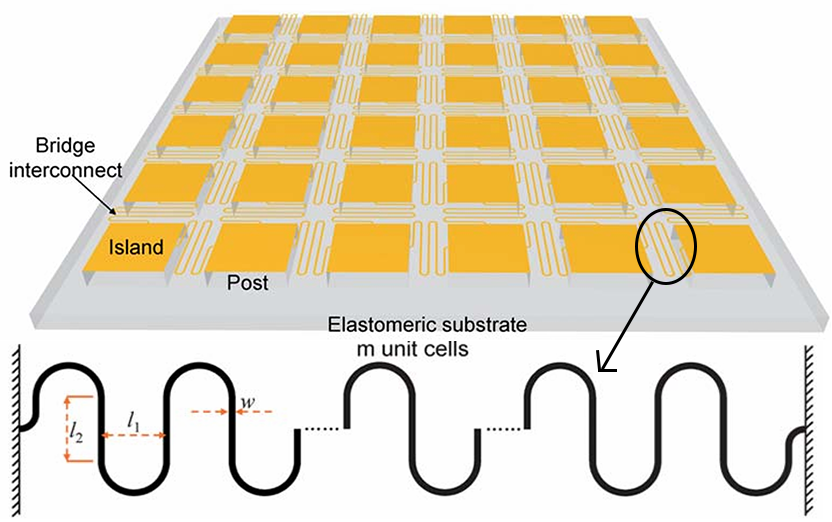
\includegraphics[width=0.6\linewidth]{1_2v.png}
	\caption{“岛—桥”布局及蛇形结构\cite{zhang2013buckling}}
	\label{fig:1_2v}
\end{figure}

蛇形结构是由若干蛇形单元构成,每一蛇形单元由直线条带与半圆弧条带相互交错连接而成\cite{li2005compliant}。相比于直线条带,蛇形条带具有更好的可拉伸性。由于蛇形条带的截面宽度远大于其厚度,面外弯曲刚度远小于平面内弯曲刚度,因此当拉伸载荷超过某一临界值时结构会发生面外屈曲。而在后屈曲阶段,蛇形结构的弹性能主要是由弯曲和扭转弹性能为主,保证了在较大拉伸下蛇形结构不会因轴向拉伸而破坏。正因为蛇形结构良好的可拉伸性,该结构已被广泛应用于各类柔性器件中,如图~\ref{fig:1_3v}所示。例如,Jiao等\cite{jiao2023vertical}通过蛇形结构连接各个电子器件来构建曲面型的电子设备;Kobayashi等\cite{Kobayashi2018FlexibleSW}通过采用蛇形条带将超薄芯片与基座连接,实现了芯片在基座上的可移动性,使芯片能够在基座上进行有限范围内的位移或旋转。Xu等\cite{xu2013stretchable}利用蛇形结构连接电池单元来制造可拉伸柔性电池。Lai等\cite{lai2017single}将可穿戴式摩擦发电单元设计为蛇形结构并安置在编织基底上,提高了该能量收集装置的可拉伸性。
\begin{figure}
	\centering
	\subcaptionbox{曲面型柔性电子设备\cite{jiao2023vertical}\label{fig:1_3(1)}}
	{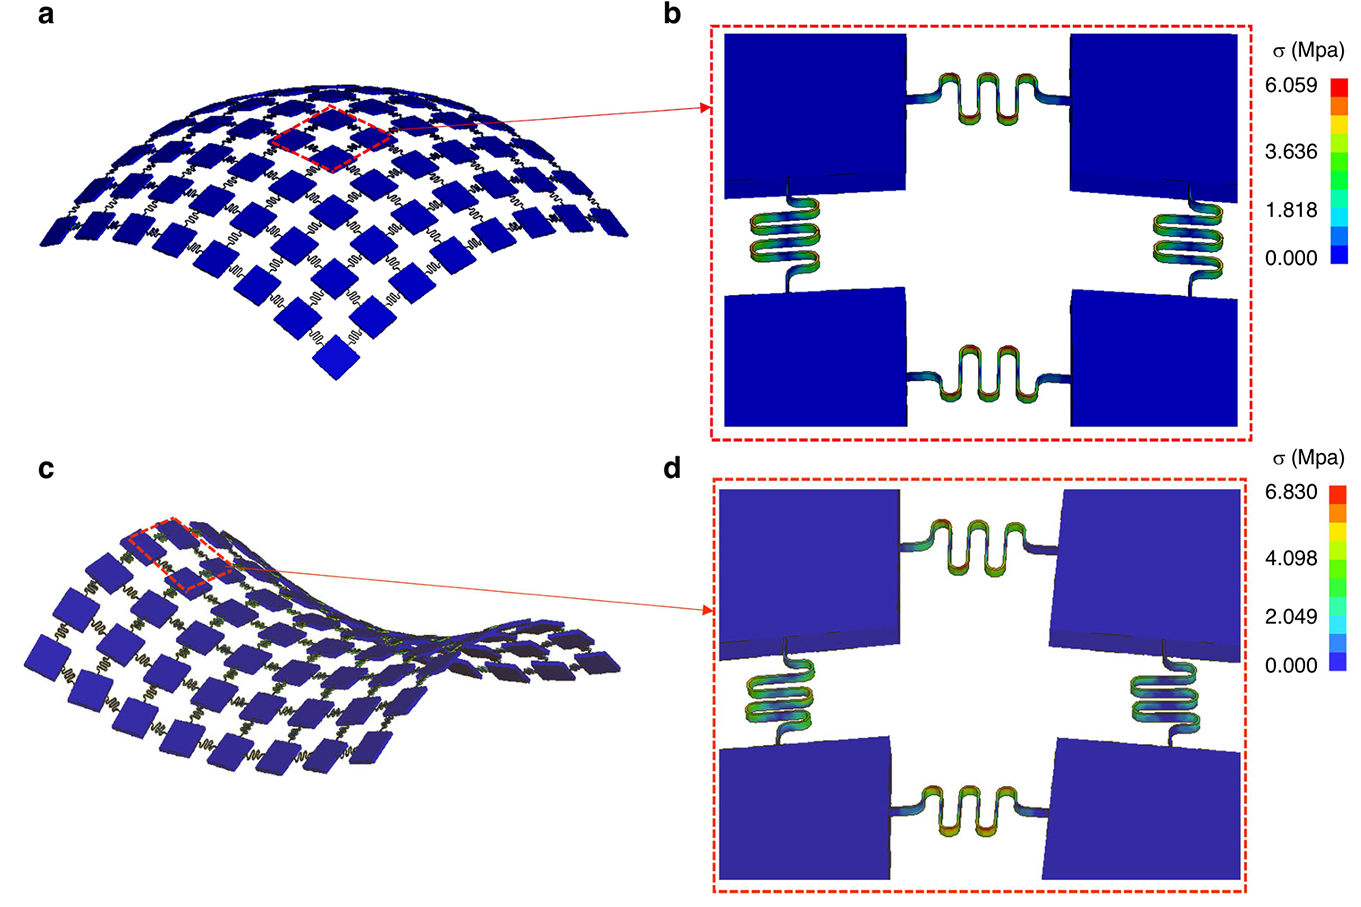
\includegraphics[width=0.45\linewidth]{1_3(3).png}}
	\subcaptionbox{可移动芯片基座\cite{PhysRevLett.99.084301}\label{fig:1_3(2)}}
	{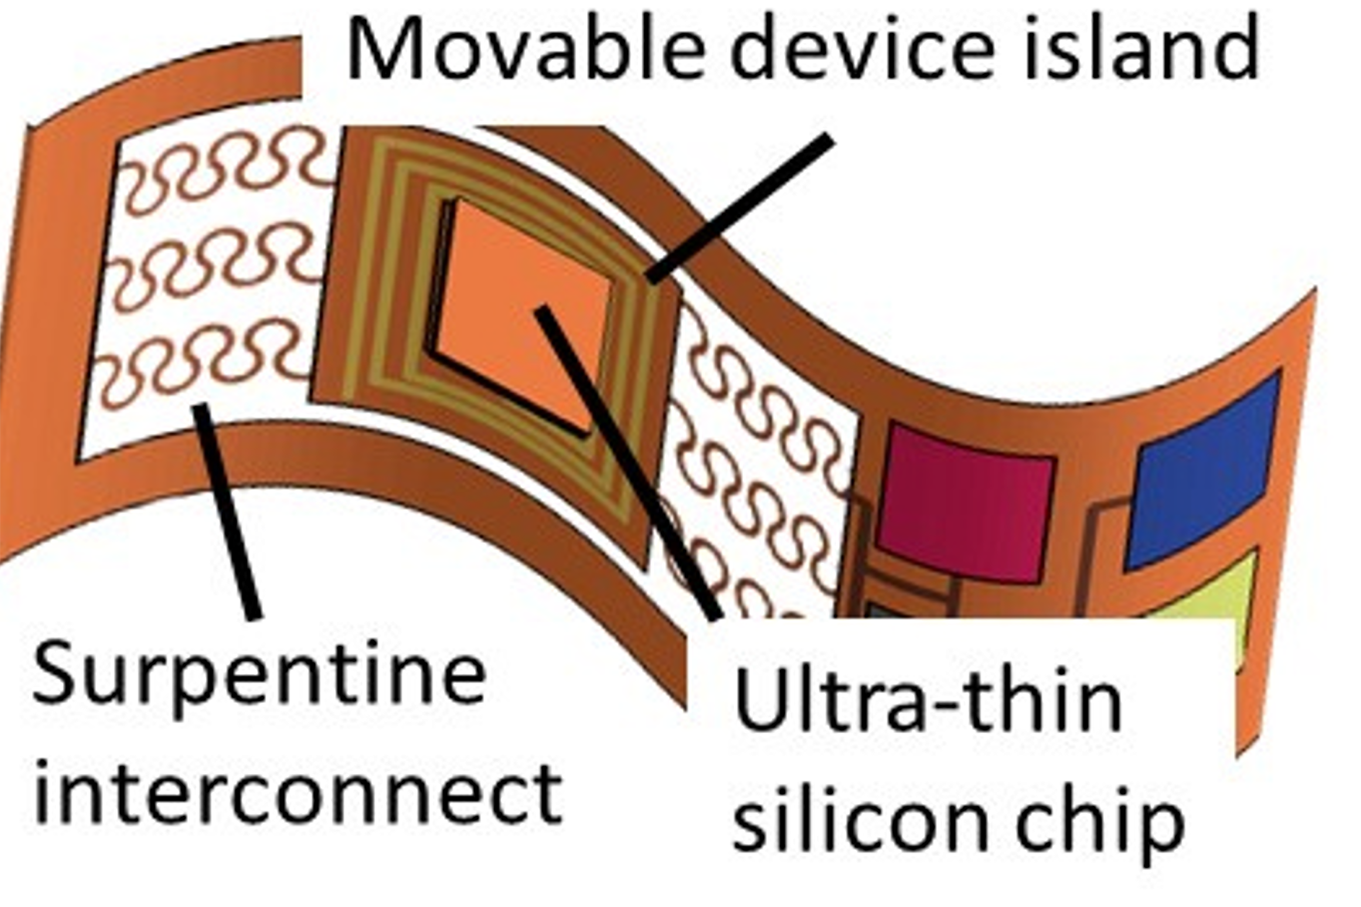
\includegraphics[width=0.45\linewidth]{1_3(4).png}}\\
	\subcaptionbox{柔性电池\cite{xu2013stretchable}\label{fig:1_3(3)}}
	{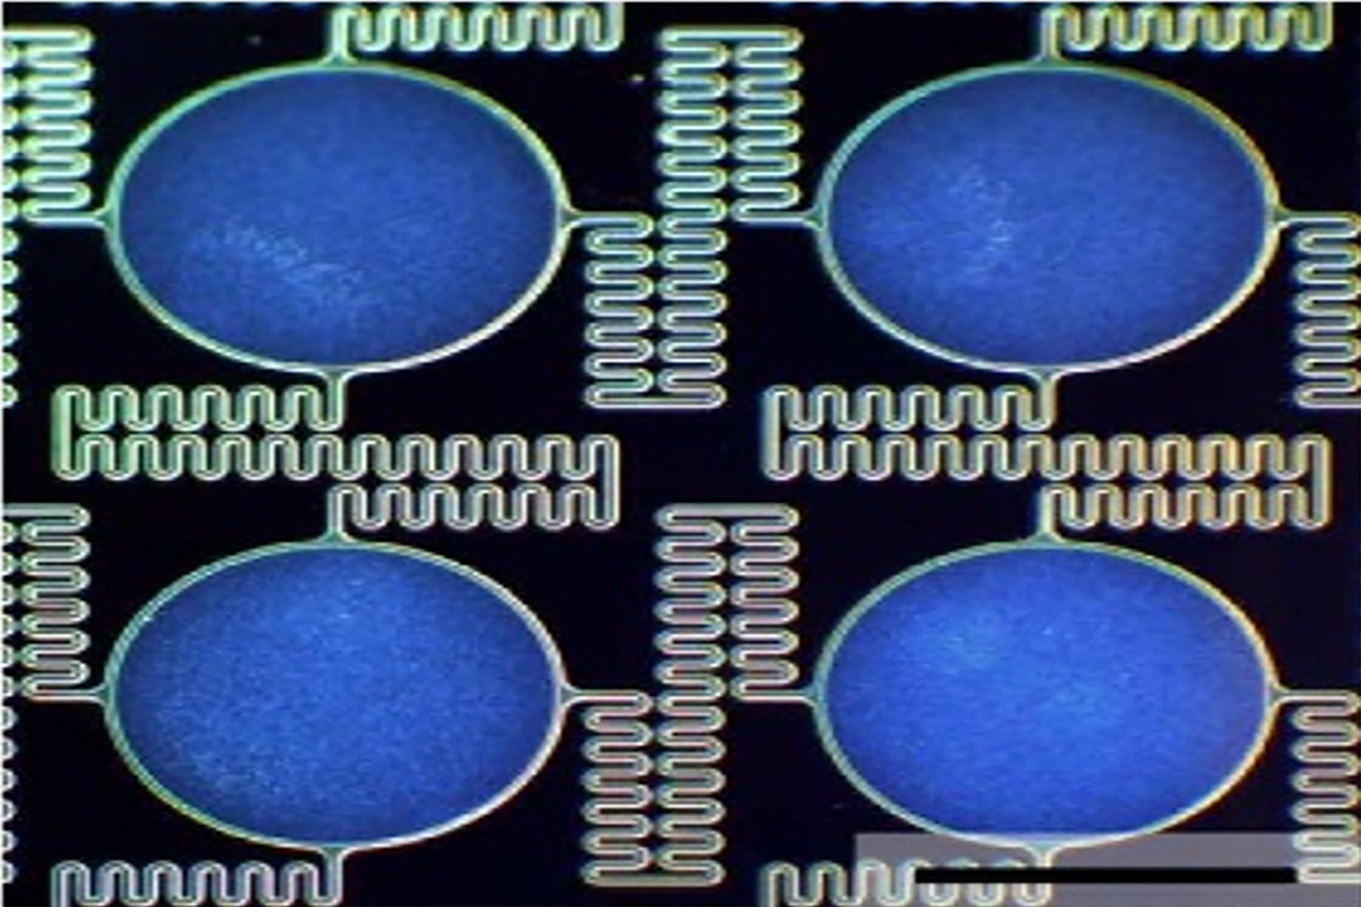
\includegraphics[width=0.45\linewidth]{1_3(2).png}}
	\subcaptionbox{可穿戴发电设备\cite{lai2017single}\label{fig:1_3(4)}}
	{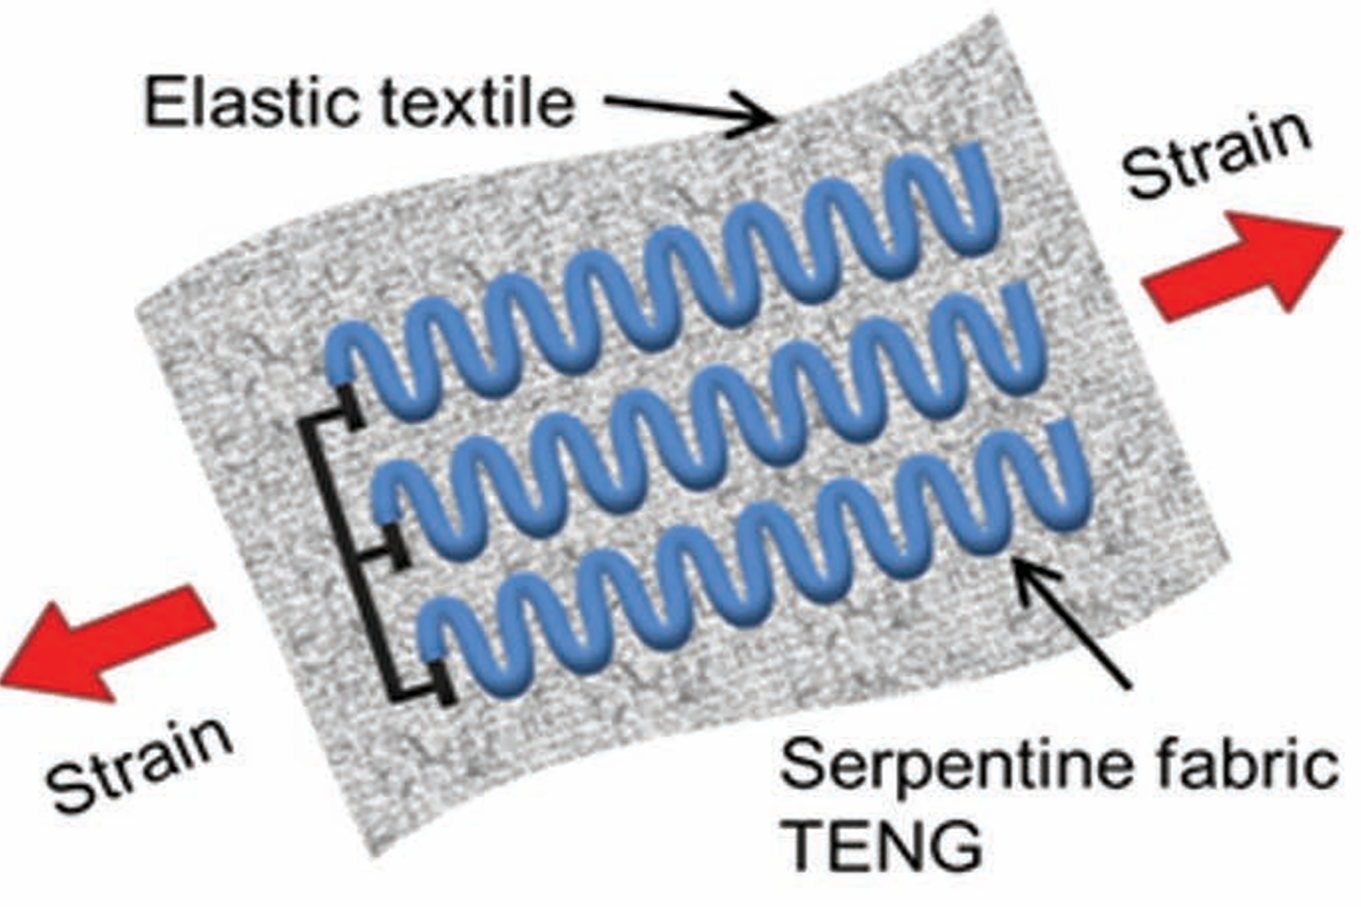
\includegraphics[width=0.45\linewidth]{1_3(1).png}}
	\caption{蛇形结构的实际应用}
	\label{fig:1_3v}
\end{figure}

综上所述,蛇形结构作为一种具有优异可拉伸性能的柔性连接部件,已被广泛应用于可拉伸柔性电子设备中。然而,目前大多数研究主要聚焦于蛇形结构的可拉伸性能,而对其在后屈曲阶段表现出的丰富非线性力学行为(如多稳态行为、稳态间突跳等)尚未充分挖掘和利用。这些非线性行为设计更为智能、自适应的柔性设备提供了潜在的可能性。例如在后屈曲阶段,蛇形结构展现出复杂的力学响应,例如多稳态特性可用于实现结构的自适应变形,而稳态间的突跳行为则可为快速响应提供新的途径。然而,目前对该结构的这些非线性行为的机理研究仍不够深入,缺乏系统的理论分析和实验验证,限制了其在工程实际中的进一步应用。因此,本文将详细研究不同单元数的蛇形结构的后屈曲行为;在此基础上提出优化调控该结构后屈曲行为的方法,为实际的应用提供理论依据,从而推动柔性电子、智能材料等领域的技术进步。


\section{国内外研究现状}
\subsection{弹性蛇形条带结构}
本小节总结了现有文献中关于蛇形条带力学行为的研究成果。基于不同的应用需求,已有研究主要聚焦于以下三个方面:在三维组装技术\cite{cheng2023programming}中,该结构受压屈曲为研究重点;作为振动测量装置时,其振动特性成为研究重点;而在柔性电子设备中,则主要关注其拉伸状态下的力学行为。因此,现有研究主要集中于该结构的受压/受拉屈曲行为及其振动响应特性。

在三维组装技术中\cite{cheng2023programming},蛇形结构常被用作构建目标三维结构的基础平面构型。该技术通过将二维结构(如蛇形条带结构)固定于预拉伸的柔性基底上,当释放基底预拉力时,二维结构将因受压而发生面外屈曲失稳,如图~\ref{fig:1_4(1)}所示。因此,深入研究蛇形结构受压屈曲的力学行为具有重要意义。Li等\cite{li2019mechanics}采用有限元方法,系统研究了蛇形结构的几何参数和材料参数与屈曲构型上最大应变之间的关系。在此基础上,Zhao等\cite{zhao2021torsional}进一步发展了一套力学模型,详细刻画了蛇形结构受压屈曲后的构型特征,包括构形曲率、挠率以及结构中应力分布等关键力学信息。

振动测量方法为表征生物材料的物理特性(如细胞质量和杨氏模量)提供了有效手段,如图~\ref{fig:1_4(2)}所示。蛇形结构受压会失稳屈曲,不同的压力载荷会诱导产生不同的屈曲构型,而每种屈曲构型又具有独特的振动响应特性。因此基于蛇形结构设计的可调谐的振动框架\cite{zhao2021theoretical},能够方便调整配置、振动模式和共振频率。基于此,众多研究聚焦于蛇形结构屈曲后的振动响应特性。例如,Zhao等\cite{zhao2023theoretical}建立了理论模型来预测蛇形结构的振动行为,并推导出了预测结构固有频率的解析表达式。
\begin{figure}
	\centering
	\subcaptionbox{蛇形结构的三维组装\cite{jiao2023vertical}\label{fig:1_4(1)}}
	{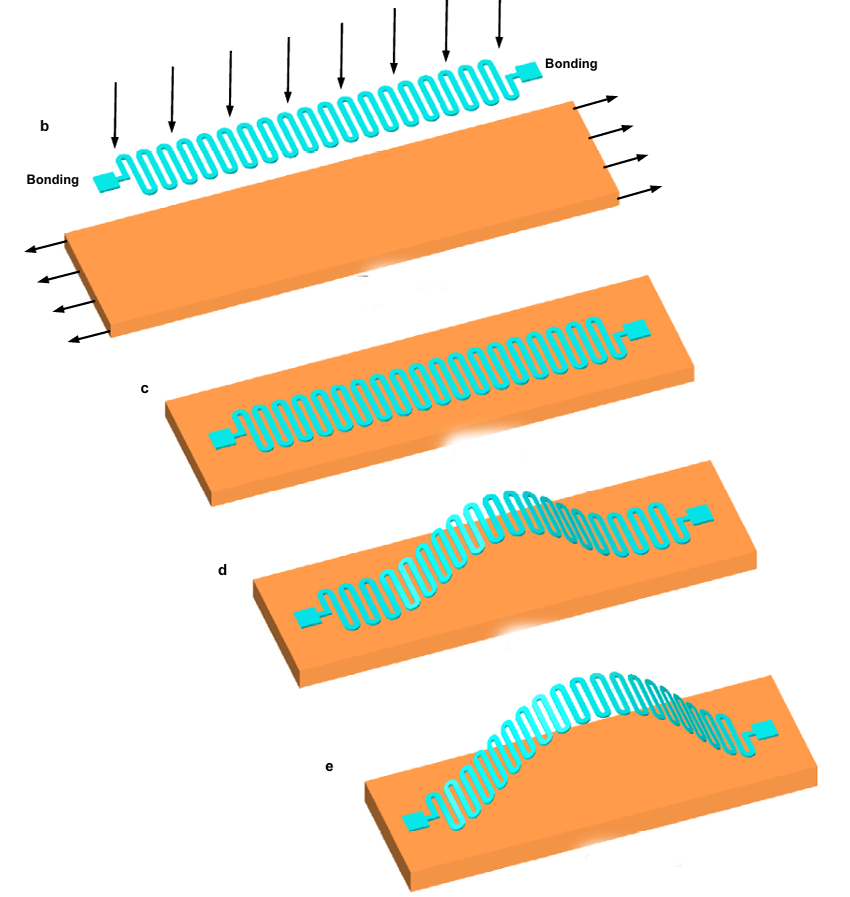
\includegraphics[width=0.45\linewidth]{1_4(1).png}}
	\subcaptionbox{蛇形结构可调谐振动测量装置 \cite{zhao2021theoretical}\label{fig:1_4(2)}}
	{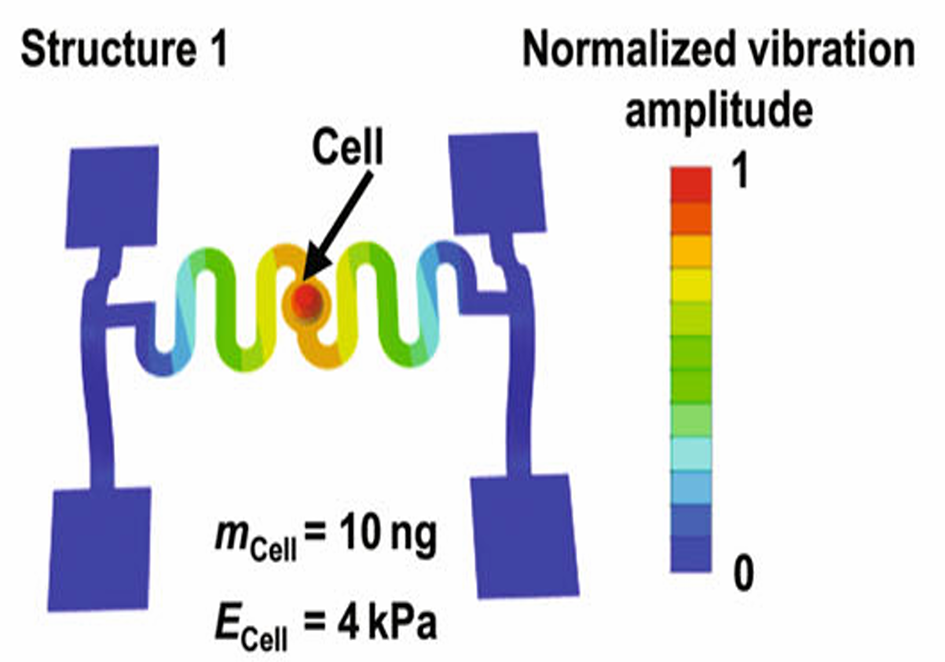
\includegraphics[width=0.45\linewidth]{1_4(2).png}}
	\caption{蛇形结构受压屈曲的应用}
	\label{fig:1_4v}
\end{figure}

对蛇形结构在拉伸载荷下力学行为的研究主要可分为两类:一类聚焦于结构未发生面外失稳时的平面解,另一类则关注结构失稳后的屈曲行为。在对平面解的研究中,Widlund等\cite{widlund2014stretchability}针对宽厚比较小(不易发生失稳)的蛇形结构,基于曲梁理论给出了的解析解,并通过有限元数值模拟验证了解析结果的准确性。Fan等\cite{fan2016finite}基于有限变形理论,提出了非线性的解析表达式,进一步完善了蛇形结构平面解的理论模型。

在对蛇形结构的屈曲行为研究中,Feng等\cite{feng2020analytical}推导了蛇形结构的无量纲临界屈曲载荷与长宽比之间的简单比例关系。Zhang等\cite{zhang2013buckling}通过有限元计算,揭示了单单元蛇形条带在两端固支的边界条件下,蛇形条带存在两类失稳模态分别为反对称稳态(如图~\ref{fig:1_5}中第二行第一列所示)和对称稳态(如图~\ref{fig:1_5}中第二行第一列所示)。随着高宽比的增加,蛇形条带失稳模态由反对称转变为正对称模态。而对于多单元蛇形结构只存在反对称稳态,如图~\ref{fig:1_5}中第一行第一列所示,其屈曲模态与高宽比无关。

通过对蛇形结构研究现状的分析可以发现,在实际应用中该结构往往处于后屈曲状态。因此,深入研究蛇形结构的后屈曲力学行为对于指导工程应用具有重要的理论和实践意义。然而,现有研究主要局限于对一阶屈曲模态的分析,对后屈曲状态下丰富的非线性力学行为的研究仍显不足。具体而言,虽然Zhang等\cite{zhang2013buckling}揭示了屈曲模态与结构高度之间的关联性,但尚未给出相应的力学机理解释。此外,该结构在后屈曲阶段表现出的多稳态特性也缺乏系统研究。基于此,本研究将系统探究蛇形结构在后屈曲阶段的非线性力学行为,重点包括屈曲模态交换机制、多稳态特性及分岔行为等关键问题。


\subsection{细长结构稳定性分析}
蛇形结构具有复杂的分岔行为,在分岔点前后平衡路径的稳定性往往会发生改变,而平衡解的失稳往往对应着结构屈曲以及结构突跳等行为,因此,准确判定平衡分支的稳定性对研究蛇形结构的非线性行为至关重要。细长结构在各种载荷和各类约束下的稳定性问题,是弹性理论最基本且最古老的问题之一,其历史可以追溯到欧拉对弹性杆的研究。目前,关于细长弹性杆稳定性分析的研究大致可分为两类:一类是静力学方法,主要基于能量最小原理进行稳定性判断;另一类则是基于动力学稳定性判断准则的方法。

静力学稳定性判断方法基于能量最小原理,根据势能理论,处于稳定平衡状态的结构其弹性能通常对应于势能函数的局部最小值。能量泛函取得最小值不仅要满足能量泛函一阶变分为零,同时也要保证二阶变分的非负性。通过考虑平衡解对应的雅可比方程\cite{gelfand2000calculus}(二阶常微分方程),若雅可比方程存在非零解,且该解在定义域中不会穿过横坐标(无共轭点),那么根据雅可比强条件,可以说明该平衡解为稳定解。Morse等\cite{morse1951introduction}证明了若在定义域的端点不是共轭点,那么定义区间内共轭点数与平衡解指数相等。因此,稳定性的判定归结为定义区间内是否存在共轭点\cite{gelfand2000calculus}(conjugate point)的判断。

对于边界条件为Dirichlet条件的保守系统而言,共轭点可以用来判断解的稳定性。Manning等\cite{manning1998isoperimetric}将共轭点测试方法用于对DNA结构的稳定性判断。同时,通过对稳定性矩阵行列式的计算,提高了判断解稳定性的计算效率。Hoffman等\cite{hoffman2002calculation}通过共轭点测试对端部受扭转的不可拉伸梁的稳定性进行了判断。提出了一种通过对特定载荷参数下(弧长1处为共轭点的载荷)共轭点测试的方法,来判断结构的稳定性,避免了在载荷参数变化后,判断稳定性需要重新求解微分方程的初值问题所带来的计算成本。

对于Neumann–Neumann边界条件的系统而言,Manning等\cite{manning2009conjugate}将通过共轭点测试判断结构稳定性的方法推广到Neumann–Neumann边界条件的情形。在该文章中讨论了有限维系统的海森矩阵的谱与二阶变分算符的谱的关系。

另一种稳定性判断方法则是基于动力学稳定性准则。Goriely等\cite{goriely2000nonlinear}通过在三维细长结构平衡解附近施加扰动的方法来判断结构在该平衡解的稳定性。通过摄动法,对平衡解加入扰动项,线性化扰动方程,提出了动力学变分方程,用来判断解的稳定性。通过非线性的分析得到了幅值方程,用来描述失稳后的动力学行为。该文章通过非线性Klein-Gordon方程来描述初始曲率为零的细长杆失稳后的运动模式。

Kumar等\cite{kumar2010generalized}根据动力学稳定性判据,对细长结构的动力学方程通过有限元进行离散,离散后对系统稳定性的判断归结为奇异矩阵的广义特征值问题。该文章提出了一种求解奇异矩阵的广义特征值的算法,从而进行稳定性的判断。该方法可以处理更加广泛的边界条件,包括积分约束条件,多点约束条件。

Liu等\cite{liu2011stability}在动力学Cosserat模型下,通过给螺旋线在平衡解处施加扰动的方法研究螺旋线的稳定性,给出了失稳的临界载荷。揭示了Lyapunov稳定性概念和欧拉稳定性概念在细长结构稳定性判断上的区别,Lyapunov稳定性判断为稳定的解,实际上已经发生了屈曲。对于螺旋线而言,在空间域上的Lyapunov和欧拉稳定性条件是在时间域上Lyapunov稳定性条件的必要条件。

由于静力学判定能量泛函极小值的方法对载荷以及边界条件有较大限制,且该方法仅适用于保守系统,对存在非保守力(阻尼力以及跟随力)的系统而言,该方法难以进行稳定性的判定。因此,本文利用动力学系统稳定性概念来对细长结构进行稳定性分析,设计一种算法来对任意曲率的细长结构在任意载荷下的稳定性进行有效判定。
\subsection{结构屈曲行为调控}
结构优化是工程设计中不可或缺的重要环节,其目标是在满足各种约束条件的前提下,寻找最优的结构设计方案。例如,在航空航天领域,往往需要在满足刚度强度等要求下,对结构进行轻量化设计。另外,一些研究者致力于设计多层级结构(同时存在微结构与宏观结构)来实现结构更为良好的特性以及设计多功能材料。为此,目前已发展出包括拓扑优化\cite{jihong2021review}在内的许多结构优化方法来对结构进行优化设计。

蛇形结构被广泛应用于柔性电子设备中,为了满足不同柔性设备的要求,同样需要对该结构进行优化设计。蛇形条带结构良好的可拉伸性是其被广泛应用于柔性电子设备的主要原因,因此一些研究通过优化蛇形结构参数来提高其可拉伸性能,例如,Ye等\cite{ye2022automatic}系统地探讨了蛇形结构的几何参数和材料参数与其最大拉伸应变之间的关系,并提出了相应的优化策略。另外,蛇形条带结构在使用过程中的形变往往会影响结构的导电性能以及信号传输能力\cite{han2022electrical}。其中,Gutruf等\cite{gutruf2014strain}研究了具有不同圆弧段角度的蛇形微电极的电阻应变敏感性。鉴于蛇形结构在承受拉伸载荷时通常处于后屈曲状态,且根据本文实验结果表明该结构在后屈曲阶段表现出显著的非线性行为,因此,通过优化设计手段来调控蛇形结构,以充分利用其非线性特性从而实现更优的性能显得尤为必要。目前,针对该结构的优化研究主要聚焦于其可拉伸性,而对其后屈曲行为的优化尚未得到充分关注。为此,本文将提出一种优化方法,旨在有效调控蛇形结构的后屈曲行为。

过去对结构失稳屈曲行为的优化调控中,主要集中在两个方面,一方面通过优化方法来提高结构的临界失稳载荷,以避免工程结构的失稳,而另一方面,通过优化方法,来调控结构的屈曲构形。在以提高临界失稳载荷为优化目标的优化设计中,往往需要进行特征值分析来决定失稳载荷,例如,Maalawi等\cite{maalawi2002buckling}对具有各种截面形状的柔性杆的截面面积进行优化,给出了多种提高临界失稳载荷的设计方案。Wang等\cite{wang2017buckling}和Wu等\cite{wu2015framework}利用利用优化方法来对网格加筋复合板中的加强纤维的排布方式进行设计,来提高复合板的临界屈曲载荷。不同于以上研究,Lindgaard等\cite{lindgaard2011unified}通过追踪复合材料壳结构的非线性平衡路径,并检测分岔点拐点的出现来得到临界失稳载荷,该方法可以给出更为准确的临界失稳载荷。随后,通过优化这些失稳点的位置以提高临界失稳载荷。

结构在后屈曲阶段展现出的丰富非线性行为可以用来设计多功能结构,因此,一些研究开始聚焦于板壳等薄壁结构在后屈曲阶段的行为并进行优化设计,例如,Li等\cite{li2019harnessing}研究了夹杂对软质多孔结构后屈曲行为以及弹性波在该介质中传播的影响。该研究说明通过改变结构的材料和几何性质,可以有效调控结构的后屈曲模态。Lanzi等\cite{lanzi2006post}通过将有限元与遗传算法(genetic Algorithms)以及全局优化算法来对处于后屈曲范围内的复合材料板进行优化以提高其失效对应的最大载荷。Bochenek等\cite{bochenek2006structural}基于粒子群优化算法来优化结构屈曲后的平衡路径,通过优化结构参数使得结构的平衡路径沿着预定轨迹行进。

本文基于Lindgaard等\cite{lindgaard2011unified}的优化思路,将优化对象由临界失稳载荷对应的分岔点拓展到后屈曲阶段的各类分岔点以实现对后屈曲行为的调控。具体而言,本文中借鉴了对动力系统优化的一种方法:通过优化分岔点的数量及位置来调控动力系统行为\cite{melot:hal-04378993}。本文将该优化策略应用于对蛇形结构后屈曲行为的调控,以实现对蛇形结构的优化设计。
\subsection{研究现状总结}
从上述分析可知,尽管过去对弹性蛇形条带的研究已较为深入地分析了一阶屈曲模态特性,但对其后屈曲状态下表现出的多稳态切换、模态交换等非线性力学行为仍缺乏系统性探索。在蛇形结构的优化方面,现有优化设计主要集中于通过调整几何参数提升结构的可拉伸性,而针对后屈曲行为的主动调控策略尚未建立,这限制了蛇形结构在柔性电子等领域的性能优化。为此,本研究通过实验与数值模拟相结合的方法,系统研究蛇形结构在后屈曲阶段的非线性力学行为,研究成果将为蛇形结构的进一步应用提供了理论基础与设计策略。

\section{主要研究内容与研究方案}
Zhang等\cite{zhang2013buckling}发现单单元蛇形条带的屈曲模态随结构高度的变化而不同,具体而言,当高度小于某一临界高度时,其屈曲构形的二维俯视图表现为反对称形式,如图~\ref{fig:1_5}中第二行第一列所示;而当高度超过该临界值时,屈曲模态则转变为正对称构形,如图~\ref{fig:1_5}中第一行第一列所示,更为清晰的正反对称构形见图~\ref{fig:SM_Mode}。然而,对于多单元蛇形结构,其屈曲构形始终表现为反对称形式,如图~\ref{fig:1_5}中第二三列所示。本文将聚焦于这一现象并揭示该现象背后的机理。此外,基于实验观察,本文发现该结构表现出显著的多稳态特性,因此将进一步对这一多稳态行为展开系统性研究。本文通过数值计算与实验相结合的方法,对该结构进行了详细分析,并对数值结果与实验结果进行了相互验证,以确保研究结论的准确性与可靠性。
\begin{figure}
	\centering
	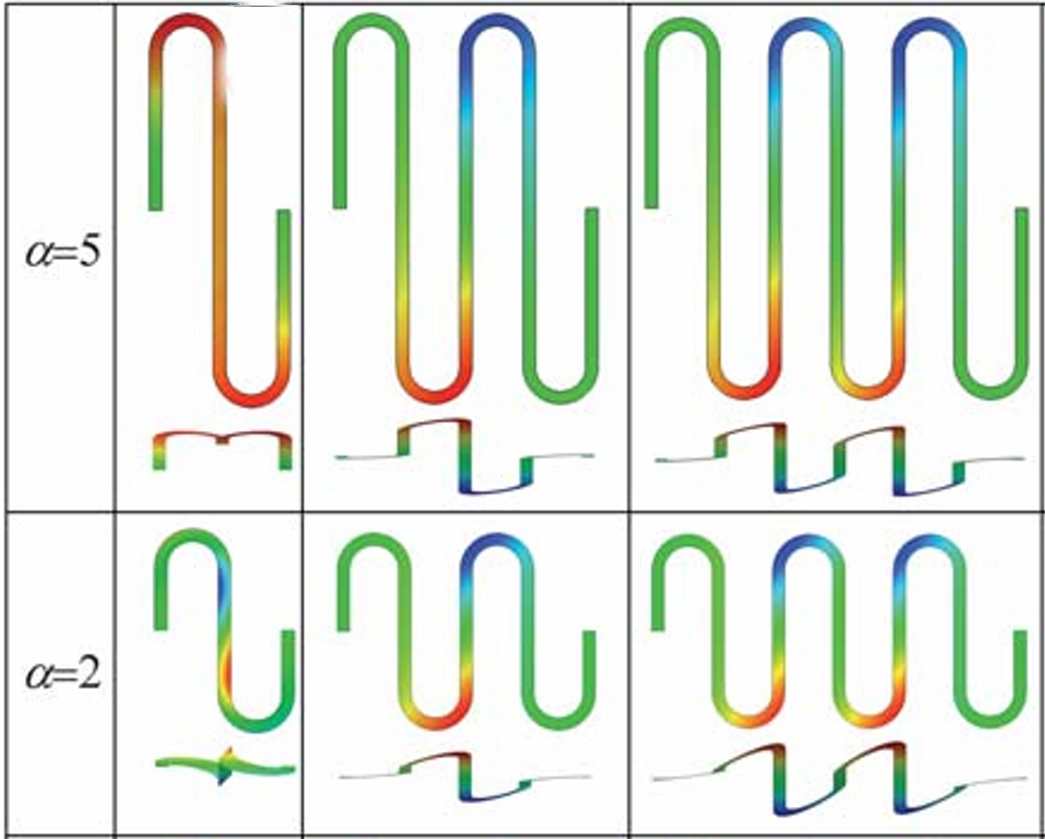
\includegraphics[width=0.6\linewidth]{1_5.png}
	\caption{不同高度,不同单元数的蛇形结构的屈曲模态,图中每一方格内下方图为屈曲模态的二维俯视图\cite{zhang2013buckling}}
	\label{fig:1_5}
\end{figure}

本文首先选取了合理的力学模型对蛇形结构进行建模。具体而言,本文采用了静力学基尔霍夫弹性杆模型\cite{dill1992kirchhoff},该模型忽略了条带结构的拉伸应变能,将条带结构简化为不可拉伸杆。已有研究表明,这种不可拉伸杆模型能够精确捕捉细长条带结构(包括由条带构成的网状结构)的非线性行为\cite{yu2019bifurcations,yu2021numerical}。因此本文将用基尔霍夫杆模型对蛇形结构进行建模,所建立的数学模型为适定的边界值问题。

为了求解此边界值问题并研究该结构的后屈曲行为,本文采用参数延拓法来跟踪平衡路径并判断分岔点的出现\cite{yu2019bifurcations,ahsan2022methods},利用MatLab分岔分析工具包COCO\cite{dankowicz2013recipes}以及分岔分析软件ATUO 07P\cite{doedel2007auto}来求解此边界值问题,并以水平拉伸位移载荷作为延拓参数,跟踪不同载荷下的平衡路径并进行分岔分析。

通过上述的分岔分析可以获得平衡路径,但在无法得到平衡分支上解的稳定性信息。平衡解的失稳往往诱发结构屈曲或平衡态突跳等非线性现象,发展一套有效的细长结构稳定性分析数值方法对蛇形条带力学行为的研究具有关键意义。本文基于动力学稳定性准则进行解的稳定性判定,为此需建立蛇形条带的动力学控制方程。这里采用离散弹性杆(Discrete Elastic Rod,简称DER)动力学模型\cite{jawed2018primer}建立初值形式的动力学方程。通过求解其不动点并计算相应雅可比矩阵来实现稳定性分析。需要特别说明的是,尽管离散弹性杆模型同样也可以对结构进行静力学分析,但离散弹性杆模型中包含了杆的拉伸应变。对于长细比极大的蛇形条带而言,拉伸应变可以忽略不计,需满足不可拉伸条件。为此,利用离散弹性杆模型对条带结构的建模过程中将拉伸刚度视为罚因子,拉伸能项视为罚函数。然而数值结果表明,过大的拉伸刚度将导致病态刚度矩阵的出现,引发数值奇异;而适度罚因子虽能保证计算稳定性,却会引入较小的误差,影响解的精度。为克服这一矛盾,本文提出混合建模策略:采用基尔霍夫杆理论进行平衡分支求解,该模型严格满足不可拉伸假设且能准确描述几何非线性效应;同时利用DER模型进行稳定性分析。

在对蛇形结构多稳态特性的研究方面,本文采用动力学离散弹性杆模型进行动力学模拟,以捕捉结构从一种稳态构形向另一种稳态构形的突跳行为。具体而言,当结构在拉伸载荷下处于某一平衡构形时,通过在该构形上施加适当的扰动力,该结构将从这一平衡构形突跳到其他平衡构形,随后在阻尼的作用下,蛇形结构会逐渐稳定到新的构形上。

蛇形条带结构几何参数的优化设计以及对其屈曲模态的调控在实际应用中具有关键意义。因此,本文在详细研究蛇形条带结构后屈曲行为的基础上,提出一种调控蛇形结构后屈曲行为的方法。该方法通过优化蛇形结构的几何参数,实现对分岔点位置及屈曲模态的主动调控,从而为结构的精确设计提供理论依据。具体而言,在保持结构对称性的条件下,将蛇形结构不同分段的条带厚度以及高度作为优化参数,使用优化工具包NLOPT\cite{NLopt}优化分岔点位置,从而实现结构后屈曲行为的调控。对于单单元蛇形条带,优化目标为调控正对称模态与反对称模态之间的临界高度。对于双单元蛇形条带,优化目标为实现一阶屈曲模态与二阶屈曲模态顺序的交换,进一步验证单单元蛇形结构与双单元蛇形结构中模态交换现象具有相同的数学机理。此外,通过调节蛇形结构的单元厚度,本文进一步揭示了单元厚度的变化能够有效影响结构的屈曲构形,这一发现为屈曲构形的精细化调控提供了新的设计维度。

综上所述,本文中所要研究的问题可阐述如下:
\begin{enumerate}
	\item 正如原始研究\cite{zhang2013buckling}中观察到的情况(一阶屈曲模态随高度增大先后为反对称、正对称),是什么导致了蛇形条带屈曲模态的交换?
	\item 在后屈曲阶段,如何通过数值计算的手段来识别其多个稳定的屈曲构形?
	\item 如何通过几何形状来调控屈曲模式以及临界屈曲载荷?
\end{enumerate}

为了解决上述问题,本文所采用的研究方法主要为:
\begin{enumerate}
    \item 基于动力学稳定性判据来判定条带结构的平衡解的稳定性。
	\item 采用基尔霍夫杆模型对蛇形结构进行建模,并利用分岔分析工具包COCO以及AUTO 07P进行分岔分析。
	\item 采用动力学模拟来研究蛇形结构的多稳态行为。
	\item 通过优化蛇形结构的几何参数,实现对分岔点位置及后屈曲行为的主动调控。
\end{enumerate}

